\mnDifficult
\begin{slikaDesno}{fig/comb_snaga.pdf}
    \PID
    У колу са слике познато jе 
    $R = 25\unit{\Omega}$ и 
    $C = \dfrac{1}{\uppi} \unit{\upmu F}$.
    Напон побудног генератора jе 
    $v_{\rm G} = \Upphi_0 \III_T (t)$, где су 
    $T =100\unit{\upmu s}$ и 
    $\Upphi_0 = 1\unit{\upmu Wb}$. 
    У колу jе употребљен и идеалан филтар пропусник опсега учестаности чиjа су централна
    учестаност 
    $f_c = 20\unit{MHz}$, ширина пропусног опсега 
    ${\rm BW} = 1\unit{kHz}$ и улазна импедансa 
    $Z_{\rm u} \to \infty$. 
\end{slikaDesno}

\begin{enumerate}[label=(\alph*)]
    \item Одредити амплитудски спектар сигнала $v_{\rm X}(t)$ и скицирати га.
    \item Одредити напон на пријемнику $R_{\rm p} = 50\unit{\Omega}$ у временском домену $v_{\rm p}(t)$, и израчунати 
    средњу снагу која се на њему ослобађа. 
    
\end{enumerate}

\RESENJE

Фуријеова трансформација побудног сигнала, може се одредити помоћу развоја у Фуријеов ред из
задатка \refz{dirak_povorka}, $\FS{\III_T(t)} = \dfrac{1}{T}$, и применом везе Фуријеовог  
реда и трансформације периодичног сигнала\footnote{Из додатка
\ref{d:CTFT}, 
$
X(\jj\upomega) = 2\uppi \sum_{k = -\infty}^{\infty} X[k] \updelta( \upomega - k \upomega_{\rm 0} )
$
}, у облику 
\begin{equation}
    \FT{v_{\rm G}} = V_{\rm g}(\jj\upomega) = 2\uppi  \sum_{k = -\infty}^{\infty} \underbrace{\dfrac{\Upphi_0}{T}}_{\mathclap{\FS{v_{\rm G}}}} \updelta( \upomega - k \upomega_{\rm 0} )
    = {\upomega_0 \Upphi_0}\III_{\upomega_0}(\upomega), \qquad \upomega_0 = \dfrac{2\uppi}{T}
\end{equation}
Такав побудни сигнал побуђује $RC$ коло па се одзив може наћи множењем спектара. 
Функција преноса $RC$ кола налази решавањем кола у комплексном домену, 
као разделник две комплексне импедансе, на основу чега је  
\begin{eqnarray}
    V_{\rm X}(\jj\upomega) = \dfrac{ \dfrac{1}{\jj\upomega C} }{ R + \dfrac{1}{\jj\upomega C} } V_{\rm G}(\jj\upomega)
                           = \underbrace{\dfrac{ 1 }{ \jj\upomega RC + 1 }}_{H_{RC}(\jj\upomega)} V_{\rm G}(\jj\upomega)
                           = \dfrac{ {\upomega_0 \Upphi_0} }{ \jj\upomega RC + 1 } \III_{\upomega_0}(\upomega)
\end{eqnarray}
%
\begin{figure}
    \centering
    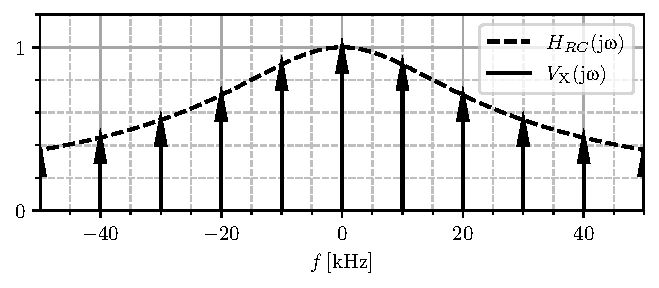
\includegraphics{fig/comb_snaga_result.pdf}
    \caption{Дијаграм функције преноса $RC$ кола, и амплитудски спектар $|V_{\rm X}(\jj\upomega)|$ }
    \label{fig:\ID.vx}
\end{figure}
%
Тражени дијаграм представљен је на слици \ref{fig:\ID.vx}. На истој слици приказана је и функција преноса $RC$ кола
$H_{RC}(\jj\upomega)$ која „обликује“ периодичну поворку импулса која представља спектар побудног напона $v_{\rm G}(t)$.

(б) Спектар напона на потрошачу одређује се множењем спектра $V_{\rm X}(\jj\upomega)$ са преносном функцијом 
идеалног филтра пропусника опсега учестаности 
$G(\jj\upomega) = 
\begin{cases}
    1 &, |\upomega - \upomega_{c}| < {\rm BW} \\
    0 &, \text{иначе} 
\end{cases}$. Можемо приметити да је пропусни опсег филтра довољно узак, тако да обухвата само Диракове импулсе на учестаностима 
$\pm20\unit{kHz}$, односно на тај начин се селектује само простопериодична компонента на тој учестаности, чиме се има 
\begin{eqnarray}
    V_{\rm X}(\jj\upomega) G(\jj\upomega) &=& 
    \dfrac{ {\upomega_0 \Upphi_0} }{ \jj\upomega RC + 1 } \III_{\upomega_0}(\upomega)
    \cdot
    \begin{cases}
        1 &, |\upomega - 2\upomega_c| < \dfrac{\upomega_0}{10} \\
        0 &, \text{иначе} 
    \end{cases} \\  &=&
    \dfrac{ {\upomega_0 \Upphi_0} }{ 1 + \jj2\upomega_0 RC  } \updelta(\upomega - 2\upomega_0)
    +
    \dfrac{ {\upomega_0 \Upphi_0} }{ 1 - \jj2\upomega_0 RC  } \updelta(\upomega + 2\upomega_0), 
\end{eqnarray}
при чему је искоришћено својство одабирања Дираковог импулса. Заменом датих бројних вредности 
налази се $2\upomega_0 R C = 1$ па се добијени израз може уредити у одговарајући облик табличних трансформација 
\begin{eqnarray}
    V_{\rm p}(\jj\upomega) &=& 20\uppi \unit{mV} 
    \left(
        \underbrace{\dfrac{1}{1 + \jj}}_{\mathclap{\frac{1-\jj}{2}}} \updelta(\upomega - 2\upomega_0)
        +
        \underbrace{\dfrac{1}{1 - \jj}}_{\mathclap{\frac{1+\jj}{2}}} \updelta(\upomega + 2\upomega_0) 
    \right)\\
    &=&
    10 \unit{mV}
    \biggl[ 
        \underbrace { \uppi \bigl(\updelta( \upomega + 2\upomega_0) + \updelta( \upomega - 2\upomega_0) \bigr) }_{
            \text{ \reft{T:ctft:cos} : } \cos(2\upomega_0 t)}
        +
        \underbrace { \jj \uppi \bigl(\updelta( \upomega + 2\upomega_0) - \updelta( \upomega - 2\upomega_0) \bigr) }_{
            \text{ \reft{T:ctft:sin} : } \sin(2\upomega_0 t)}
    \biggr],
\end{eqnarray}
па је онда коначно\footnote{Користи се 
$A \sin(x) + B\cos(x) = \sqrt{A^2 + B^2} \cos\left(x - \arctg\dfrac{B}{A} \right)$.
}
$v_{\rm p}(t) = 10\sqrt2 \unit{mV} \cos\left( 2\upomega_0 t - \dfrac{\uppi}{4} \right)$. Тражена снага потрошача онда се може 
израчунати као $P_{\rm p} = \dfrac{V_{\rm p}^2}{2 R_{\rm p}} = 2 \unit{\upmu W}$, где је $V_{\rm p}$ амплитуда простопериодичног напона.

Систем илустрован у овом задатку може се користити за умножавање учестаности. Полазећи од прецизног осцилатора познате учестаности 
тај сигнал се може пропустити кроз неки нелинеарни систем чиме ће се добити богат фреквенцијски садржај излазног сигнала. Ускопојасним 
филтрирањем неког од тих хармоника, може се добити прецизан сигнал на вишој учестаности. На пример, генерисањем четвртке на учестаности 
$10\unit{MHz}$ филтрирањем десетог хармоника добија се сигнал учестаности $1\unit{GHz}$. Овај принцип користи се код неких појачавача 
и генератора сигнала на високим учестаностима. 